\documentclass[letterpaper, 10 pt, conference]{ieeeconf}
\IEEEoverridecommandlockouts
\overrideIEEEmargins{}
% Language
\usepackage[english]{babel}
% Graphics
\usepackage[pdftex]{graphicx}
\usepackage{adjustbox}
\graphicspath{{./figures/}}
\DeclareGraphicsExtensions{.pdf,.jpg,.jpeg,.png}
% Math
\usepackage[cmex10]{amsmath}
\interdisplaylinepenalty=2500{}
% Floats
\usepackage{booktabs,multirow}
\usepackage[caption=false,font=footnotesize]{subfig}
% URLs
\usepackage{url}
% Useful Macros
\newcommand{\fref}[1]{Fig.~\ref{#1}}
\newcommand{\tref}[1]{Table~\ref{#1}}
\newcommand{\sref}[1]{Section~\ref{#1}}
\newcommand{\code}[1]{\texttt{#1}}
\newcommand\mat[1]{\boldsymbol{#1}}
\newcommand\vect[1]{\boldsymbol{#1}}
\newcommand\matop[2]{\boldsymbol{#1}\left({#2}\right)}

\title{\LARGE \bf{}
Contact Force Estimation for Robotic Arm using Motor Currents/Torques
}

\author{Raymond Djajalaksana, Francisco Suarez, and Quang-Cuong Pham}

\begin{document}
\maketitle
\pagestyle{plain}
\thispagestyle{plain}

% Content
\begin{abstract}
Here goes the abstract...
\end{abstract}

\section{Introduction}
Introduction goes here.

\section{Model Estimation}
Model Estimation here

\section{Experimental Setup}
\subsection{Motor Current Readings}
Setup description.
\subsection{Setup}

\begin{itemize}
  \item Section reference: \sref{sec:setup} depicts the setup...
\end{itemize}

\section{Results}

\subsection{Model Identification}
Model Identification here

\subsection{Validation}
Validation here


\subsection{Figures}
\begin{figure}[!htb]
  \centering
  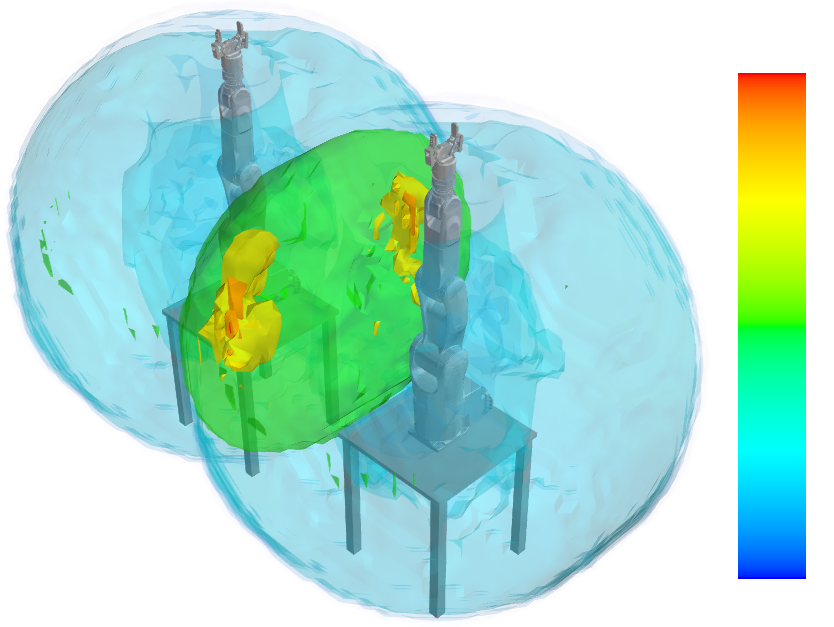
\includegraphics[width=\linewidth]{workspace};
  \caption{Normalized reachability of the bimanual setup. The workspace intersection shows the combined reachability of the two manipulators.}
  \label{fig:workspace}
\end{figure}
Appropriate values for the distance between the two robots ($d$ in \fref{fig:workspace}) can be selected either by trial and error or by solving an optimization problem with constraints imposed as a function of the resulting reachable workspace. The typical approach to quantify the manipulability of serial robots is to use a quality value for reachable positions along the robot's workspace.

\begin{figure*}[t]
  \centering
  \subfloat[$t=0$s.]{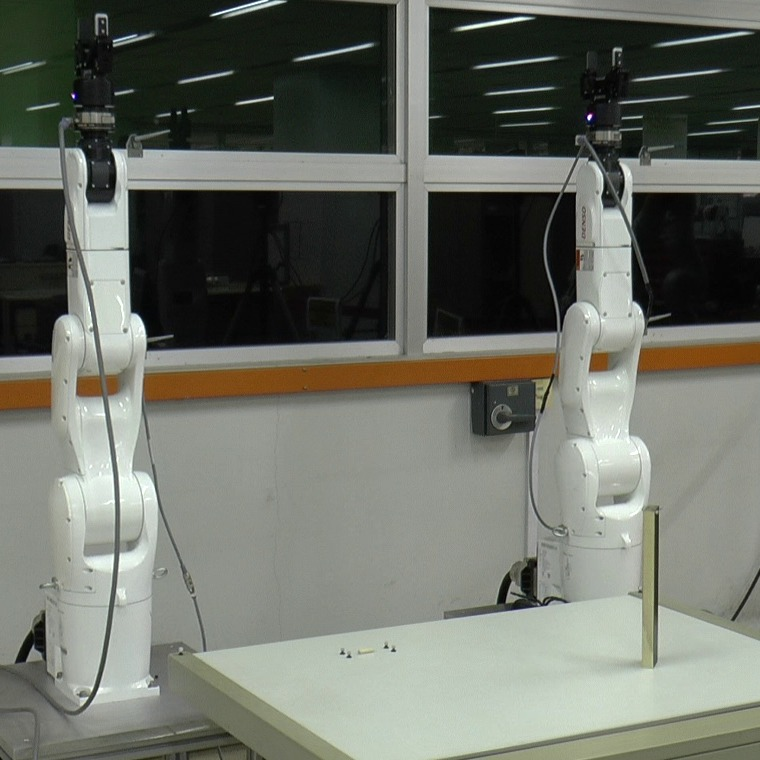
\includegraphics[height=20mm]{snapshot01}}\,
  \subfloat[$t=11$s.]{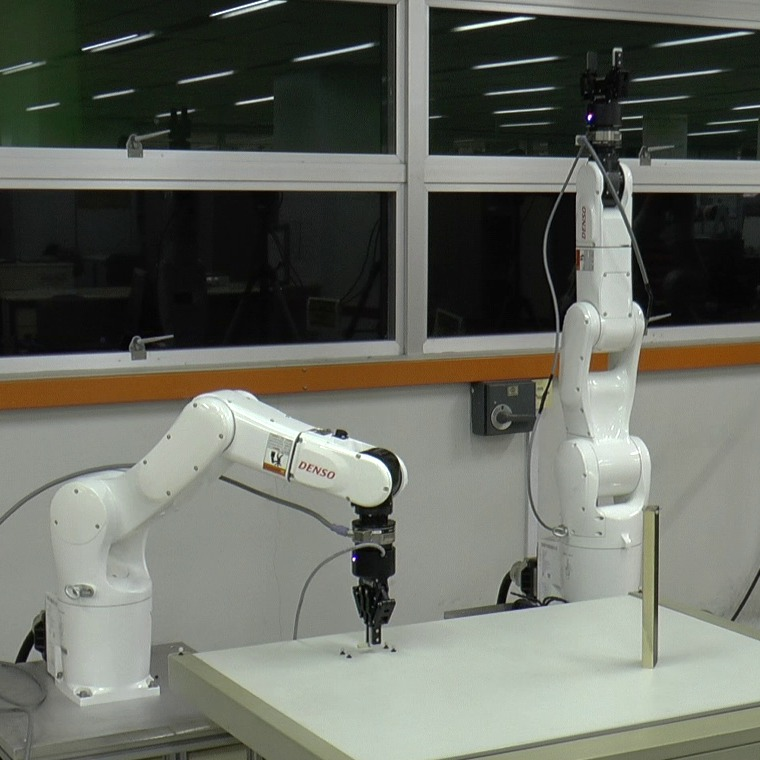
\includegraphics[height=20mm]{snapshot02}}\,
  \subfloat[$t=82$s.]{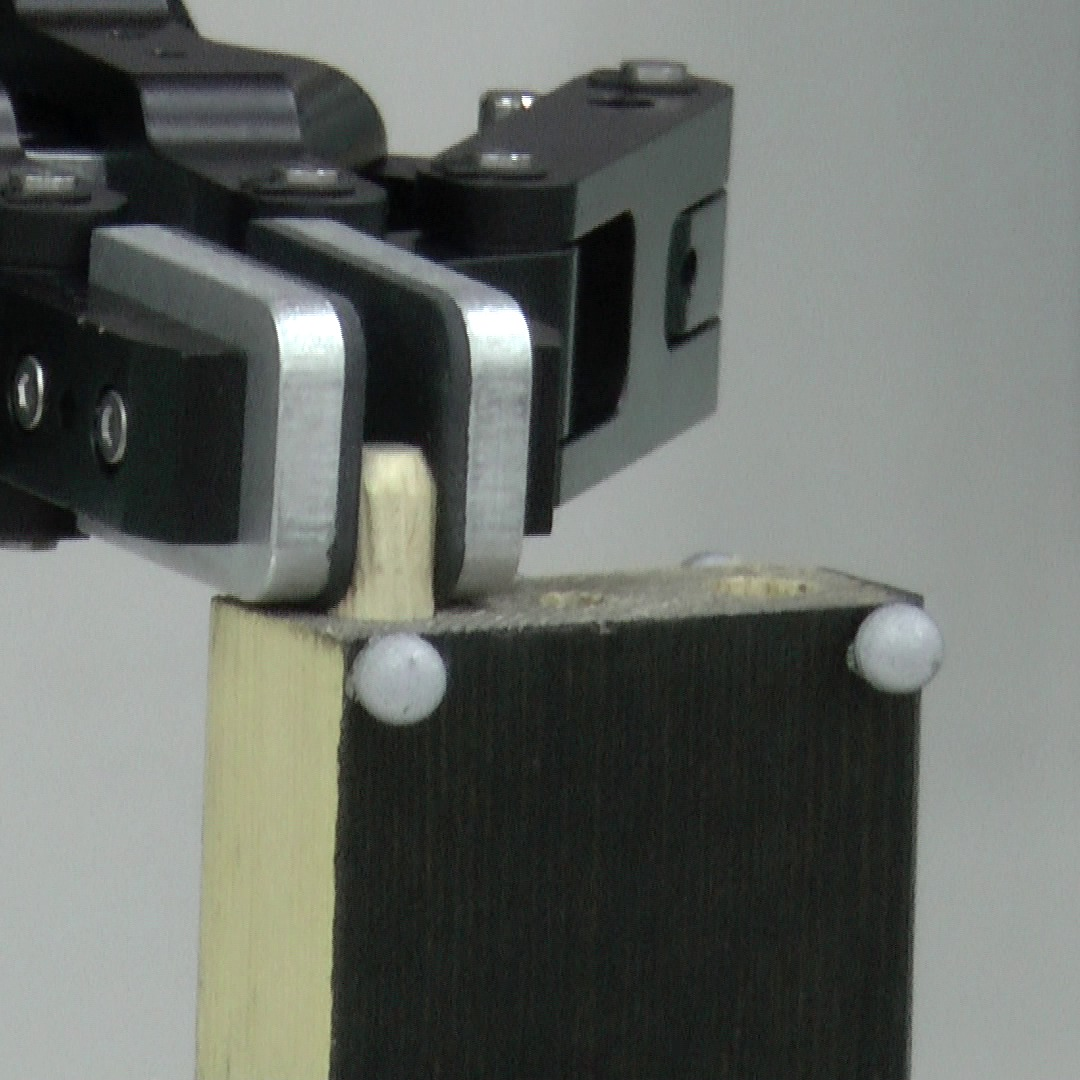
\includegraphics[height=20mm]{snapshot08}}
  \caption{Snapshots of the bimanual pin insertion. a) The initial position. The positions of the table, stick and pin are determined using the motion capture system. b) The left arm performs the compliant grasping of the pin. c) The right arm grasps the stick. d) The right arm places the stick in a position where the insertion can take place. e) The left arm moves above the stick and detects the contact with the pin. f) Through force exploration, the left arm finds the first edge of the stick. g) The left arm finds the second edge of the stick. h) Using the refined position of the two edges, the system knows where the middle axis is and can find the hole and the left arm inserts the pin. The complete video can be found at \protect\url{http://goo.gl/cYl9sq}.}
  \label{fig:snapshots}
\end{figure*}
\fref{fig:snapshots} shows snapshots of the bimanual pin insertion where each sub-task can be visually identified. The complete video can be found at \url{http://goo.gl/cYl9sq}.

\subsection{Equations}

... we use the penalization function \eqref{eq:penalization} proposed in \cite{Dubey1995},
\begin{equation}
  P(\vect{q}) = \sum_{j=1}^{n}\dfrac{\left( l_{j}^{+} - l_{j}^{-} \right)^{2}}{4 \left( l_{j}^{+} - q_{j} \right)\left( q_{j} - l_{j}^{-} \right)} \, ,
  \label{eq:penalization} 
\end{equation}

The excitation trajectory for each joint has been chosen as a finite sum of harmonic sine and cosine functions, similar to \cite{Swevers2007,Kubus2008}. Each one with a total of $2N + 1$ parameters, which correspond to the degrees of freedom of the optimization problem.
\begin{align}
  q_{j}\left(t\right) &= \sum_{k=1}^{N}{\dfrac{a_{j}^{k}}{w_{f}k}\sin\left( w_{f}kt \right) - \dfrac{b_{j}^{k}}{{w_{f}k}}\cos\left( w_{f}kt \right)} + q_{j}^{0} \\
  \dot{q}_{j}\left(t\right) &= \sum_{k=1}^{N}{a_{j}^{k}\cos\left( w_{f}kt \right) + b_{j}^{k}\sin\left( w_{f}kt \right)} \\
  \ddot{q}_{j}\left(t\right) &= \sum_{k=1}^{N}{-a_{j}^{k}w_{f}k\sin\left( w_{f}kt \right) + b_{j}^{k}w_{f}k\cos\left( w_{f}kt \right)} \, .
\end{align}
The coefficients $a_{j}^{k}$ and $b_{j}^{k}$ are the amplitudes of the sine and cosine functions. $q_{j}^{0}$ is the offset of the position trajectory.

\bibliographystyle{IEEEtran}
\bibliography{IEEEabrv,references}
\end{document}
